
%(BEGIN_QUESTION)
% Copyright 2014, Tony R. Kuphaldt, released under the Creative Commons Attribution License (v 1.0)
% This means you may do almost anything with this work of mine, so long as you give me proper credit

Determine the voltages (with respect to ground) at points {\bf A} and {\bf B} in this circuit under four different conditions: both loads off, load 1 on (only), load 2 on (only), and both loads on:

$$\includegraphics[width=15.5cm]{i01133x01.eps}$$

% No blank lines allowed between lines of an \halign structure!
% I use comments (%) instead, so that TeX doesn't choke.

$$\vbox{\offinterlineskip
\halign{\strut
\vrule \quad\hfil # \ \hfil & 
\vrule \quad\hfil # \ \hfil & 
\vrule \quad\hfil # \ \hfil & 
\vrule \quad\hfil # \ \hfil & 
\vrule \quad\hfil # \ \hfil \vrule \cr
\noalign{\hrule}
%
% First row
Voltage & Both loads off & Load 1 on (only) & Load 2 on (only) & Both loads on \cr
%
\noalign{\hrule}
%
% Second row
$V_A$ &  &  &  &  \cr
%
\noalign{\hrule}
%
% Third row
$V_B$ &  &  &  &  \cr
%
\noalign{\hrule}
} % End of \halign 
}$$ % End of \vbox

\underbar{file i01133}
%(END_QUESTION)





%(BEGIN_ANSWER)

$$\vbox{\offinterlineskip
\halign{\strut
\vrule \quad\hfil # \ \hfil & 
\vrule \quad\hfil # \ \hfil & 
\vrule \quad\hfil # \ \hfil & 
\vrule \quad\hfil # \ \hfil & 
\vrule \quad\hfil # \ \hfil \vrule \cr
\noalign{\hrule}
%
% First row
Voltage & Both loads off & Load 1 on (only) & Load 2 on (only) & Both loads on \cr
%
\noalign{\hrule}
%
% Second row
$V_A$ & 26.4 volts & 26.3 volts & 22.4 volts & 22.3 volts \cr
%
\noalign{\hrule}
%
% Third row
$V_B$ & 5 volts & 4.46 volts & 4.23 volts & 3.78 volts \cr
%
\noalign{\hrule}
} % End of \halign 
}$$ % End of \vbox

%(END_ANSWER)





%(BEGIN_NOTES)

Students will have to re-consider (and possible re-draw) the circuit for each loading condition, which is one of the major points of this question.  The fact that a circuit can ``change'' just by throwing a switch is an important concept for electronics students to grasp.  

Another concept employed in this question is that of voltages specified at single points with an implied reference of ground.  Note to students how each voltage was simply referenced by a single letter, either {\bf A} or {\bf B}.  Of course there is no such thing as voltage at a single point in any circuit, so we need another point to reference, and that point is ground.  This is {\it very} commonly seen in electronic circuits of all types, and is a good thing to be exposed to early on in one's electronics education.

A much less obvious point of this question is to subtly introduce the concept of discrete states (loading conditions) available with a given number of boolean elements (switches).  Given two load switches, there are four possible states of circuit loading, previewing binary states in digital circuits.

%INDEX% Electronics review: series-parallel circuits

%(END_NOTES)


